% Activate the following line by filling in the right side. If for example the name of the root file is Main.tex, write
% "...root = Main.tex" if the chapter file is in the same directory, and "...root = ../Main.tex" if the chapter is in a subdirectory.
 
%!TEX root =  testMain.tex

\chapter[Simulations to Evaluate Bayesian Networks.]{Creating Simulations to Evaluate Bayesian Networks.}

\section{Introduction}

In this part, I explain the general method for creating simulations with automatic Bayesian Networks, as well as how to evaluate these Bayesian Networks. The general process of creating simulations to evaluate Bayesian Networks is illustrated in Figure~\ref{pipeline}. We start by defining a simulation with agents, and then have reporters report on that simulation in the `Experiment' stage. Relevant events in simulations are collected by the reporters in each run. The collection of runs is used by an automatic Bayesian Network constructor algorithm to construct a Bayesian Network automatically in the `Building BN' stage. Finally, the constructed Bayesian Network is evaluated with respect to the criteria in the `Evaluate BN' stage. These three stages are explained in this section. Specific instances of simulations and networks I created with this process are the subject of the next chapters.

\begin{figure}[h]
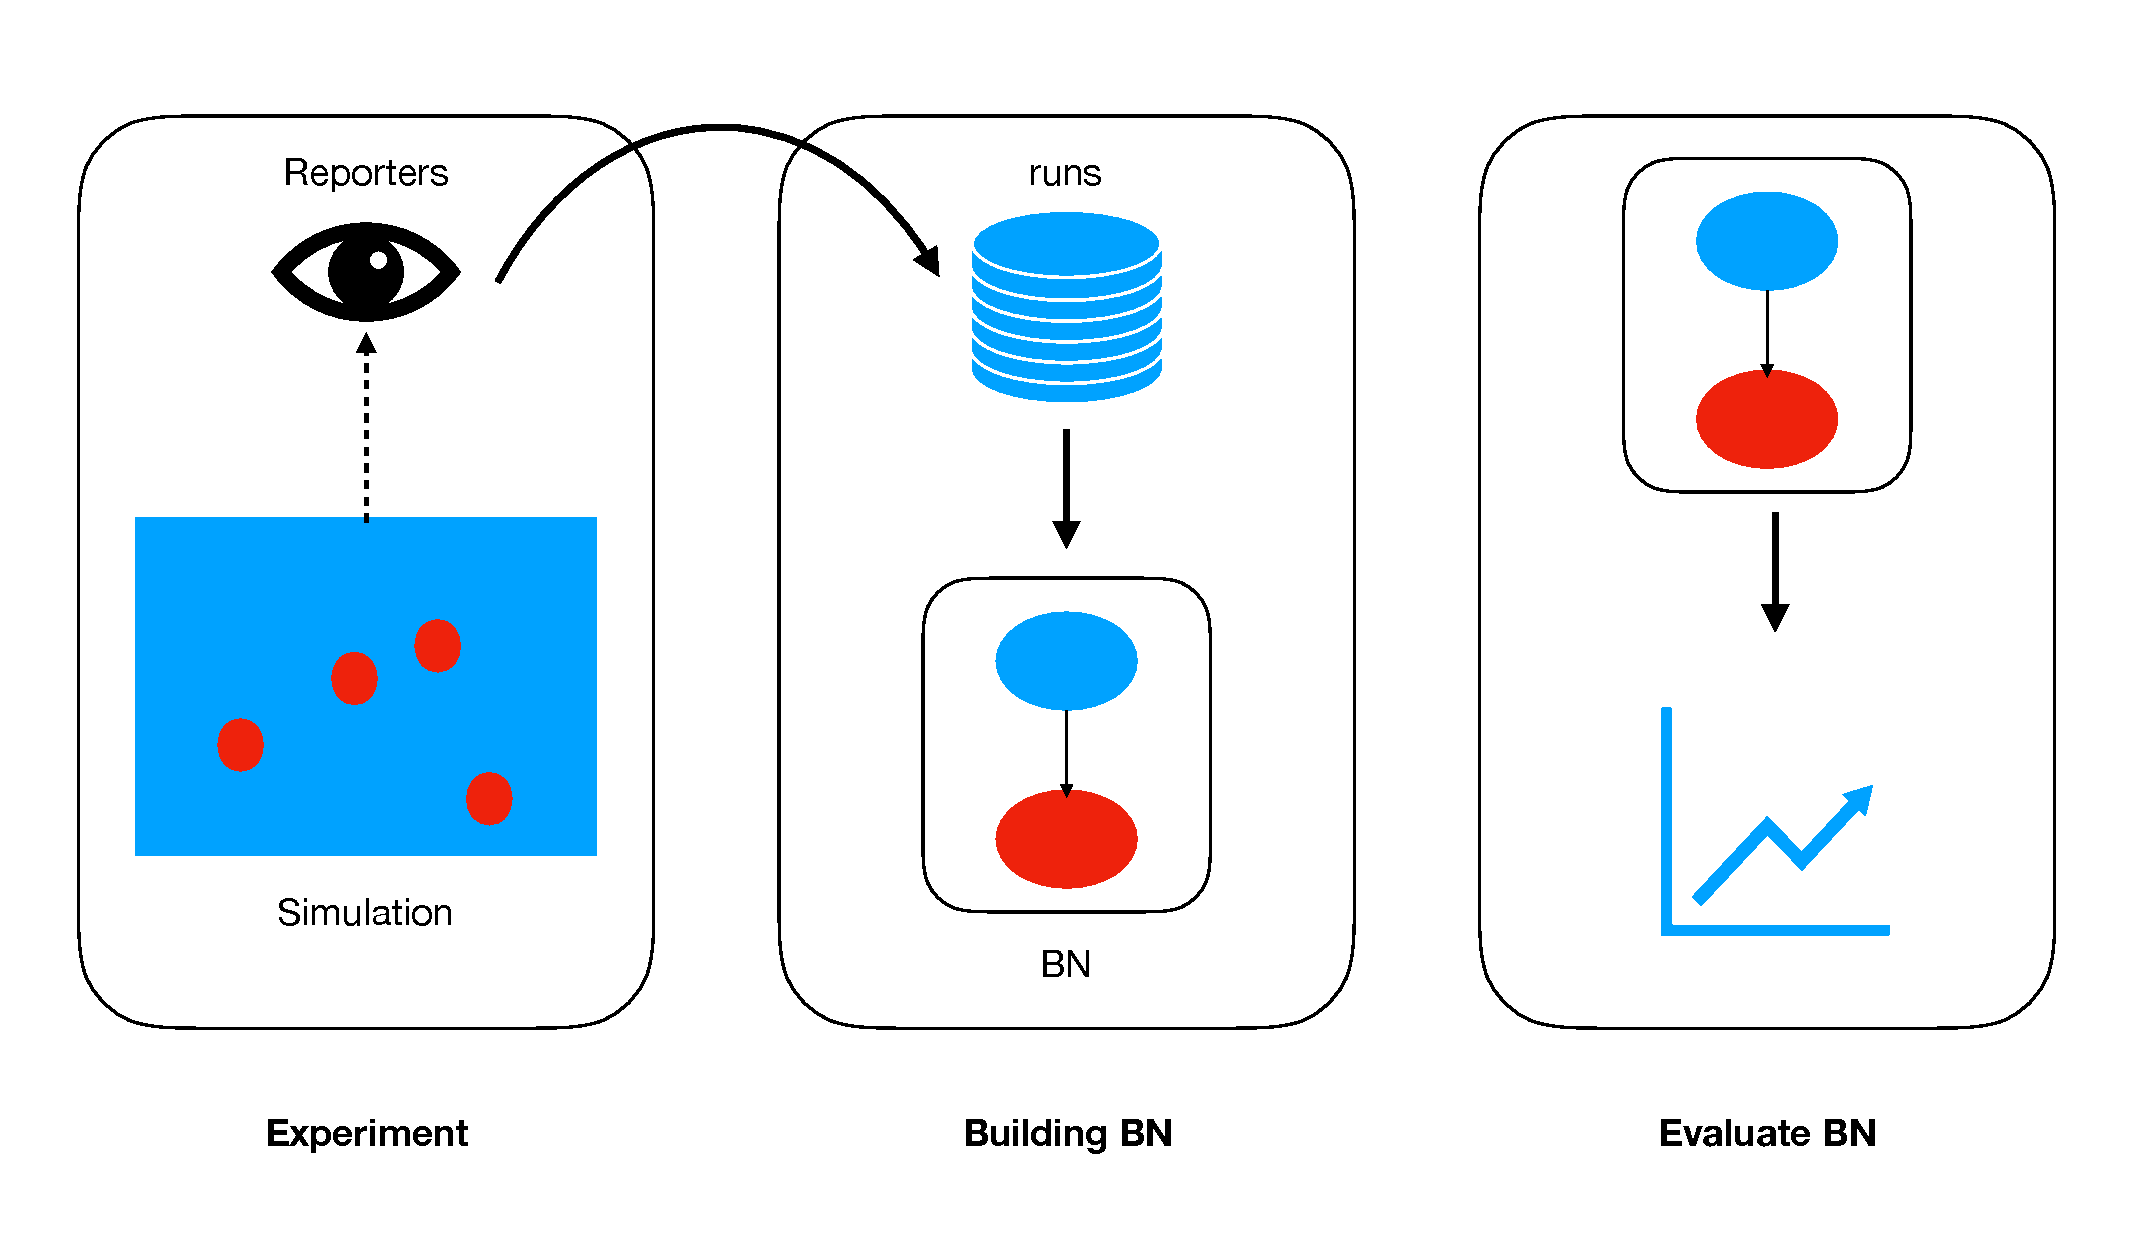
\includegraphics[width=\linewidth]{images/pipeline.pdf}
\label{pipeline}
\caption{Method for evaluating automatically generated Bayesian Networks from simulations.}
\end{figure}


\section{Setting-up an Experiment}
An experiment consists of a simulation and reporters. Reporters are defined separately from the simulation because they are not inherent to it - they are defined with respect to what we want to know about the simulation.

\subsection{Simulation}

\subsubsection{Structure of a simulation}
In the simulation, we are simulating some sort of criminal scenario - a theft, usually. Or we are simulating purely for the theoretical things. The simulation can be as precise as necessary, but there are certain things that need to be present: we need to have states that happen, there needs to be evidence for those states as well. The granularity of the simulation and its complexity depend on the modeller and her requirements.

\subsubsection{Spatial and Non-spatial simulations.}
I'm discussing two types of simulations: spatial simulations and non-spatial simulations. In a spatial simulation, an agent's behaviour is mediated with respect to their environment - eg, agents cannot pass through buildings, or cannot see agents that are far away, or can only steal from another agent when that agent is nearby. In a non-spatial simulations, agents can behave and interact with each other, but this is happening without any environment, hence we are simulating an abstraction. In concrete terms, you can think about a non-spatial simulation as a communication game.

For this project, that means that spatial simulations are more complex and interesting than non-spatial simulations, as there are more possibilities for variety.

The simulations were programmed in MESA, a python package that is made for the creation of Multi-agent systems simulations. We define an environment that the agents can interact with, as well as agents that perform some behaviours. Specifics of simulations and agent behaviour are described in the following chapters.

\subsubsection{Predictability and randomness}
Where does the interest of the simulation come from? In one part, agents sometimes do things because they are commanded to do so by the computer \footnote{rephrase, this is always true lol.}. This means that, at the start, a random number generator might `decide' that some agent has a motive, since the random number generator generated a 1 instead of a 0. On the other hand, some randomness arises from interactions between agents, or between agents and their environments. This is where spatial simulations bring additional value compared to non-spatial simulations.

 In non-spatial simulations, all agent states are essentially brought about by a combination of randomly generated numbers, and reasoning rules. For example, if an agent has a tendency to lie (randomly generated), and it has the opportunity for lying (brought about due to the current non-spatial simulation), then it will lie. Hence a combination of behavioural rules and randomly generated numbers results in a state of `agent lies' of 1.
 
 However, in spatial simulations, interactions and behavioural rules and randomly generated numbers are all brought together: if an agent is near another agent (chance interaction), and it has a tendency to steal (randomly generated), then it will attempt (but might not succeed) in stealing. Here the behavioural rule might lead to a more interesting/complex/complicated outcome than in the non-spatial simulation.
 


\subsection{Reporters (as Random Variables)}

In the simulation, certain states can be brought about. For example, an agent can succeed in stealing an object, or in lying, or in having a motivation (or in not having those things). We need a way to observe these states: this is where reporters come in. A reporter reports the outcome of a relevant event or state in the simulation, and is embedded in the code. If an event happens (or does not happen), the reporter reports that the event is true (or false). In essence, the reporter ($R$) is a random variable (RV) (for a further explanation of Random Variables, see Chapter 8!). In short, a random variable maps an event ($e$) to a truth value:

\[ R : e \rightarrow \{0, 1\} \]

Not all the states in the simulation have a reporter associated with it - otherwise I could build infinitely many reporters. I could have reporters for names, for $agent\_Q\_at\_x\_1\_y\_200$. Hence, I only created reporters for states I deemed relevant for the scenario that I am investigating. Here is a subjectivity gap. I can imagine that in my simulation of the Grote Markt (see later chapter), there is some part of the simulation that by chance geometry, lends itself to an easier job for the thief than another part of the simulation. If the thief and victim spawn near this point, then the probability of the thief succeeding will be higher. Increasing the granularity of the reporters might help us determine if there is a spot like this. However, I did not implement this level of granularity in the simulation (yet), because that is a local and specific part, and does not fit into the more global scenario description (the scenario of theft is spatially-free).

The global state of one run of the simulation, is the combination of all reporters.

\[ G = (e_0 \rightarrow \{0, 1\} \times e_1 \rightarrow \{0, 1\} \times ... \times e_n \rightarrow \{0, 1\})\]
 or,
 
\[ G = R_1 \times R_2 \times... \times R_n\]
for $n$ reporters.

Then, we collect these global states over the number of runs that we do for each experiment, which results finally that the output $O$ of this stage of the method, is a series of global states, one for each run:

\[ O = (G_0, G_1, ... G_{runs})\]


\section{Creating a Bayesian Network from a Simulation Automatically}

The output of an experiment is the collection of runs $O$, where each run is the global state $G$ of the simulation, as measured by the random variables $R$. Semantically, it fits that reporters are random variables, as the reporters become the nodes in the Bayesian Network.

Once we have a collection of states and runs, we can give this to an automated Bayesian Network learner, such as those implemented in pyAgrum. These learners can interpolate a Bayesian Network using algorithms, such as Greedy Hillclimbing and K2. This results in automatic generation of the Bayesian Network which is solely based on the data that is collected in $O$. 


K2 and temporal restraints.  No restraints on evidence (evidence can connect to each other)



\section{Evaluating the Bayesian Network}

We want to evaluate different aspects of the Bayesian Network: structural criteria, performance criteria and human criteria.

\subsection{Structural Criteria}
\begin{enumerate}
\item Hypotheses are ordered temporally. Following the cause-consequence idiom.
\item Evidence connects to hypotheses.
\item Relevance: All relevant events are in the BN, all irrelevant events are outside of the BN.
\item Independent events are not connected to each other.
\end{enumerate}

\subsection{Performance Criteria}
\begin{enumerate}
\item Accuracy.

We generate a training set of $m$ entries and a test set of $n$ entries, by running the simulation respectively $m$ and $n$ times. At every run, we collect the state of the simulation from the reporters. This results in $m$ rows for the training data and $n$ rows for the testing data. The K2 algorithm is trained on the full $m$ entries of the training set, which results in a Bayesian network. The number of runs $n$ and $m$ depend on the simulation, but $n$ is always 10\% of $m$.

The accuracy is calculated on the testing set. Every row in the testing set has a set number of elements: one element for each reporter. For every row, at random, one element in the row is obscured. The rest of the row is passed as input to the Bayesian Network, we set it as evidence. This means that there is one node that we do not set evidence on, which is the node that represents the obscured reporter. Due to the evidence now set in the network, this node now has a posterior probability. 

 We round the posterior probability to either 0 (if posterior $\leq 0.5$) or to 1 (if posterior $>0.5$). The rounded posterior is compared to the obscured element. If they match, the network has correctly predicted the state of a random reporter in the simulation. If they do not match, the network has made an incorrect prediction. The accuracy is calculated as \[\frac{correct}{total}\]


\item Root Mean Squared Error.

Similar to accuracy, except that we do not round the posterior probability. We also calculate the root mean square error as a way to see how close the posterior of the network is to the state of the world. For each row compute \[\sqrt{\frac{\sum_i^N (state_i - posterior_i)^2}{N}}\] 

\item Correspondence.

To what extend do the probabilities found in the Bayesian Network correspond to the frequencies encountered in the simulation? 

\item Sensitivity Values of Output Node.

The sensitivity analysis on the network is difficult. In essence, a sensitivity analysis's goal is to see how small changes in a conditional probability table (cpt) of a node can result in changes in some target node. Since Bayesian Networks have many parameters per node, it is not trivial to perform a sensitivity analysis that takes into account all the nodes in the network, and interpret the results in a meaningful way - this would be an $n$-way sensitivity analysis \citep{gaag2007}.  Instead, in this project, we chose to perform one-way sensitivity analyses from any node in a network to the ultimate outcome node, using Hugin's Parameter Sensitivity Wizard. This tool allows us to calculate the maximal sensitivity value of each node with respect to the ultimate outcome node. 

A sensitivity value is the first derivative of the sensitivity function, at the point of the probability value \footnote{this is a terrible explanation}. It represents how much the sensitivity function changes at the point (sensitivity functions only take certain shapes, hyperboles and linear). A sensitivity value of near 0 means that at the point of the cpt, a `small' change in the parameter would result in an infinitesimally small change in the output probability - eg, this cpt is not sensitive at all, and a misestimation might not matter so much. However, a large sensitivity value means that the value is very sensitive to change - a small change in cpt might result in a meaningfully different output. What counts as a large sensitivity value I arbitrarily decide to be $>0.5$.



\item Evidence updates the posterior in the correct direction.

Given a plausible set of evidence (for instance, the set of evidence that a lawyer might present), that we update in chronological order, does the value of the posterior of our ultimate output node change in a meaningful way (corresponding to the evidence strength with regards to the output node).

\end{enumerate}

\subsection{Human Criteria}
\begin{enumerate}


\item How robust is the network against a loss of precision? \citep{Druzdzel2013}.

We generated only one Bayesian Network, with the data we collected from the simulation. Then, we create many new networks, with this network as a basis. We do not change the number of nodes (we do not leave out or add nodes), nor the structure of the Bayesian network. We only change the values in each node's conditional probability table (cpt). In this case, we round the values in the cpt's, such that the BN becomes increasingly less precise. The intuition behind this is, that when expert users are going to elicit the probabilities, we do not know how robust the network is against smaller and larger imprecisions in the elicited probabilities. By simulating such imprecisions, we can compare the accuracy and rmsq error of the more imprecise networks to the ground truth of the `real' network. 

We round every value in the cpts $c$ to each of \[i, i \in \{\text{no disturbance}, 0.05, 0.1, 0.125, 0.2, 0.25, 0.33, 0.5\} \] according to \[ floor(\frac{c}{i} + 0.5) \cdot i.\]

\item Could a human find these probabilities?

\item Can a human determine the correct independence relations?

\end{enumerate}

Now that we've established how the automatically generated Bayesian Networks are going to be judged, we can show cautiously in the next chapter how well they are holding up!


